\chapter{Classical Machine Learning}
\label{chap:classicalml}

Twelve models were trained on the 320-feature dataset built in \Cref{chap:preprocessing}: four
algorithms, each trained three different ways. This chapter covers the algorithms, the training
modes, how a detection is scored, and these first 12 results, which were the project's baseline
for a long time. A later, wider search over augmentation methods (\Cref{chap:augmentation})
found a thirteenth model that beats every one of these --- that result is reported in full
there, not retrofitted into this chapter's original comparison.

\section{Four algorithms}

\begin{itemize}[leftmargin=1.4em]
  \item \textbf{Decision Tree} --- \texttt{DecisionTreeClassifier}, no feature scaling, default
    hyperparameters (Gini impurity, no depth limit).
  \item \textbf{Random Forest} --- \texttt{RandomForestClassifier}, no feature scaling, default
    hyperparameters (100 trees, no depth limit).
  \item \textbf{KNN} --- features standardized first, then \texttt{KNeighborsClassifier} with
    default settings (5 neighbors, uniform weighting).
  \item \textbf{SVM} --- features standardized first, then an RBF-kernel \texttt{SVC} with
    default settings (\(C = 1\), \(\gamma = \)~``scale''), with Platt scaling enabled so the
    model also outputs a calibrated probability. Platt scaling only adds this probability
    output; it does not change the underlying decision boundary.
\end{itemize}

All four pipelines use scikit-learn 1.9.1 with a fixed random seed (42) for reproducibility.
Random Forest and SVM are trained with default hyperparameters deliberately: the goal of this
project was a sound pipeline and an honest comparison across algorithms and training strategies,
not a hyperparameter search, which is left as future work (\Cref{chap:conclusion}).

\section{Three training modes}

Each of the four algorithms is trained three different ways, to address the class imbalance
established in \Cref{chap:preprocessing} head-on:

\begin{itemize}[leftmargin=1.4em]
  \item \textbf{Unbalanced.} Each training fold is used exactly as it is, with the real,
    heavily imbalanced class proportions.
  \item \textbf{Balanced.} The majority (non-seizure) class in the training fold is randomly
    undersampled down to match the seizure class, 50/50. This is repeated with 5 different
    random seeds to check how much the result depends on which non-seizure windows happen to
    get kept; seed 0 is the one used for the saved models and predictions reported below.
  \item \textbf{Augmented.} The full, unbalanced training fold, plus synthetic extra seizure
    windows built from the training recordings' own real signal. This mode is covered in detail
    in \Cref{chap:augmentation}.
\end{itemize}

In every mode, the test data is left untouched: real class proportions, real windows only, never
anything synthetic or resampled.

\section{How a detection is scored}

All 12 models are evaluated with a 5-fold \texttt{GroupKFold} split by recording, the same five
folds throughout this project: a model is never scored on a recording it was trained on. This
matters because neighboring windows from the same recording are highly correlated; splitting at
random, window by window, would let a model see near-duplicates of its test data during
training.

Scoring itself is event-level, not window-level. A window counts as positive once its predicted
probability crosses a chosen threshold; consecutive positive windows merge into one detected
interval, and nearby intervals (less than 2 seconds apart) are merged together, with anything
shorter than 2 seconds afterwards dropped as noise. A real seizure counts as \emph{found} if any
detected interval overlaps it at all; a detected interval that overlaps no real seizure counts
as a \emph{false alarm}.

\begin{figure}[H]
  \centering
  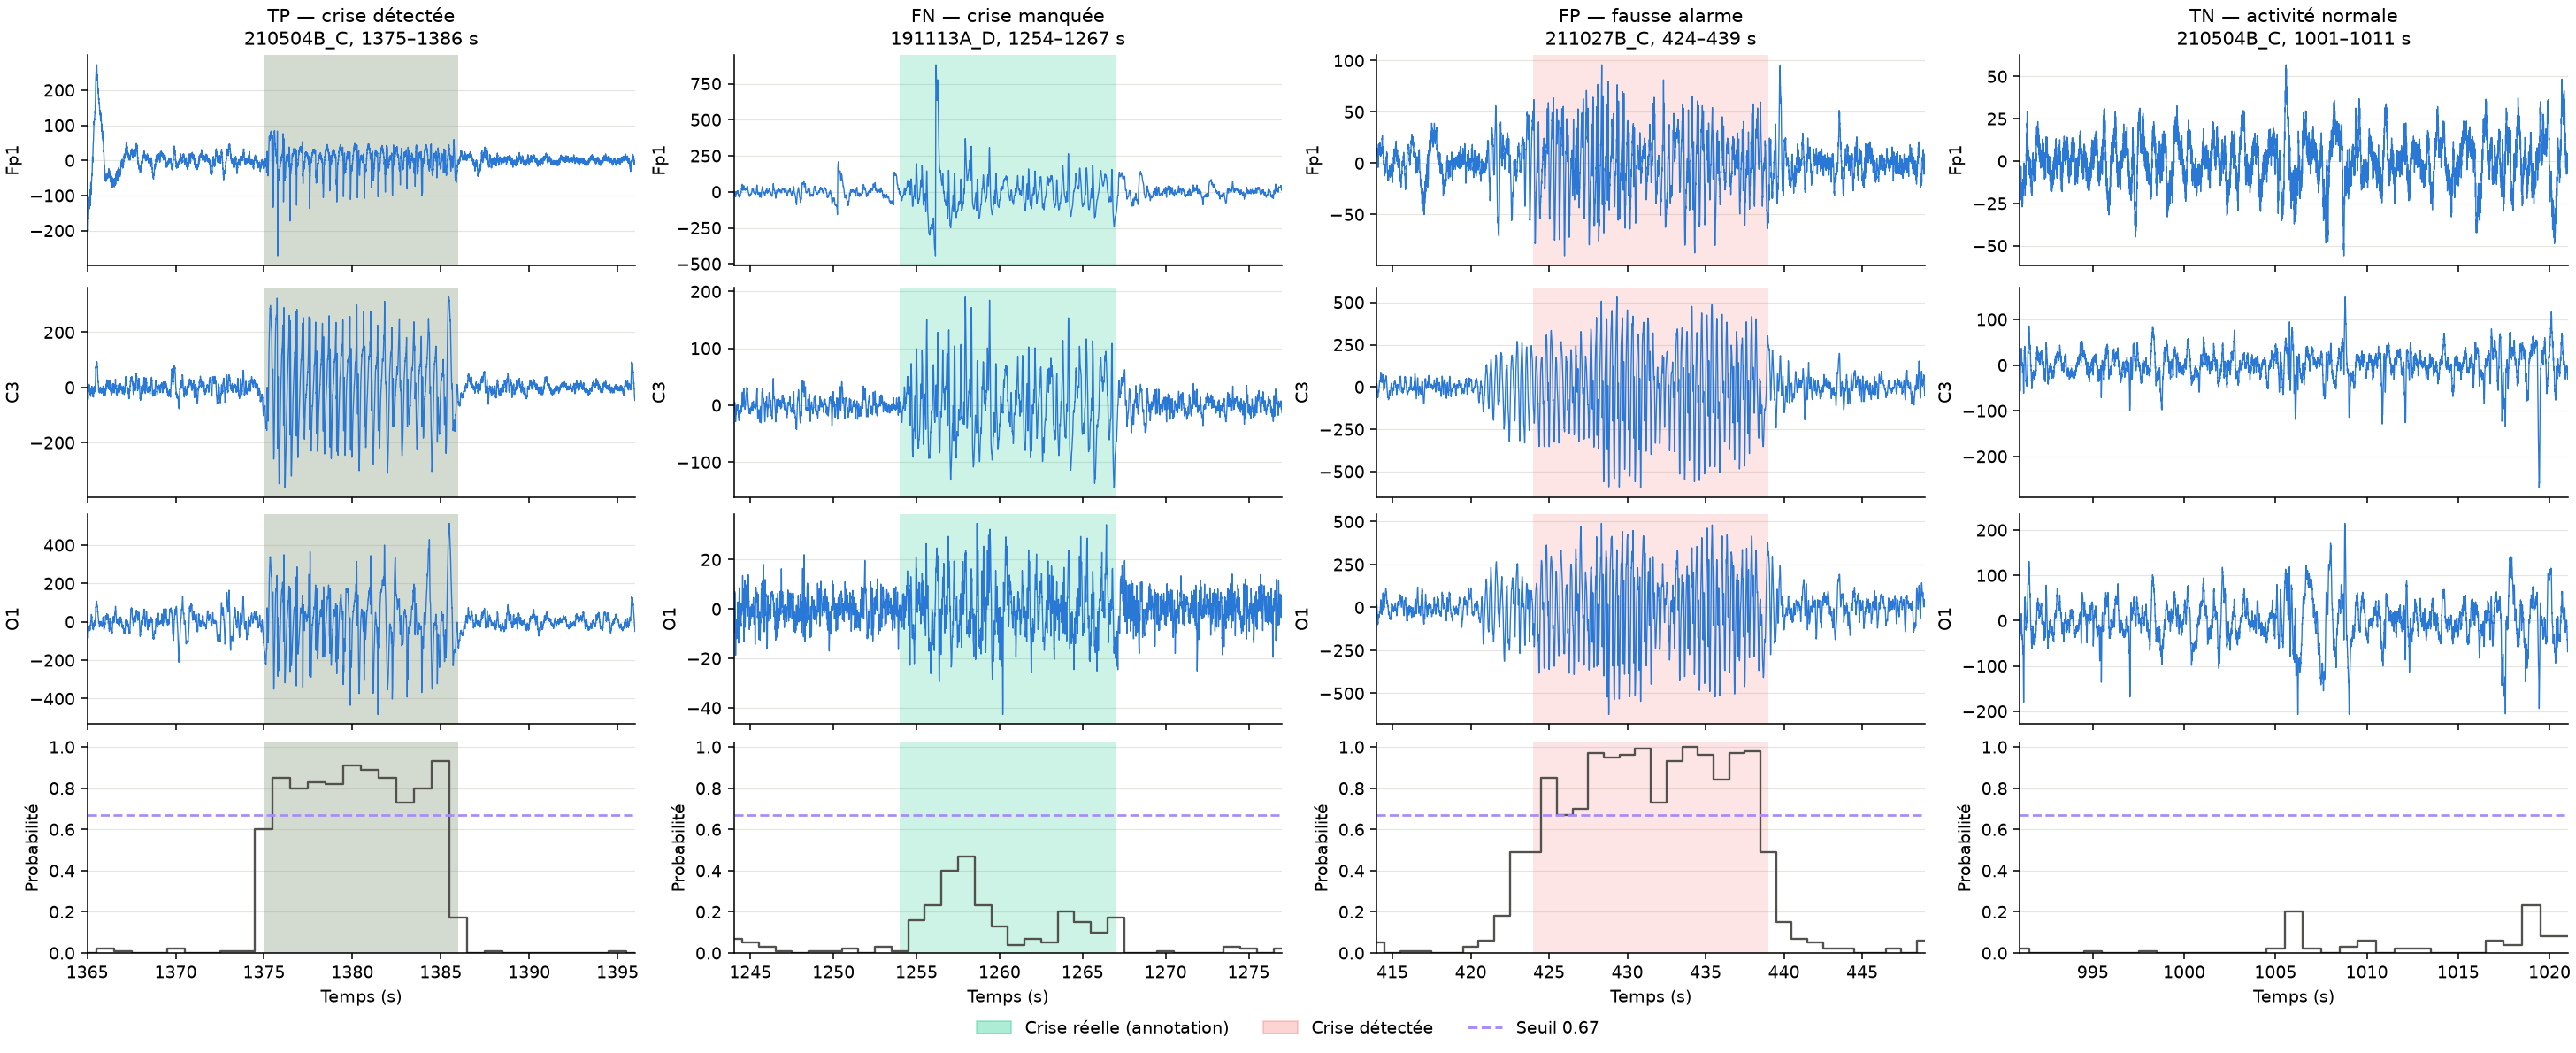
\includegraphics[width=\linewidth]{official/detection/error_examples.png}
  \caption{Four real 15-second segments from the Random Forest unbalanced model, one per
    outcome: a found seizure (TP, true positive), a missed seizure (FN, false negative), a
    false alarm (FP, false positive), and ordinary background activity correctly left alone
    (TN, true negative). Three EEG channels (Fp1, C3, O1) and the model's probability curve are
    shown for each; the dashed line is the detection threshold. Figure labels are in French in
    the original output (\emph{crise détectée} = seizure detected, \emph{crise manquée} =
    seizure missed, \emph{fausse alarme} = false alarm, \emph{activité normale} = normal
    activity, \emph{seuil} = threshold).}
  \label{fig:error-examples}
\end{figure}

The missed-seizure example is a useful reminder of what ``found'' actually requires: in that
segment, the model's probability does rise during the real seizure, but never crosses the
threshold --- a near miss, not a blind spot, and a case where a slightly lower threshold would
have caught it at the cost of more false alarms elsewhere, the exact trade-off the threshold
sweep in \Cref{chap:classicalml} is built to navigate.

Window-level accuracy is not used to judge these models: a model that never predicts a seizure
at all would still score 96\% window accuracy on this dataset, simply because seizure windows
are so rare. Event-level precision, recall, and F1 are the metrics used throughout this report.

For each model, a threshold is swept to find the one that maximizes event-level F1 on that
model's own out-of-fold predictions. Because the same predictions are used both to choose the
threshold and to score it, this ``best threshold'' number is slightly optimistic --- a caveat
carried through to \Cref{chap:evaluation}, where it matters for comparing fairly against the
deep-learning results.

\section{Results}

\Cref{tab:classical-results} gives every model's result at its own best threshold.

\begin{table}[H]
  \centering
  \small
  \caption{All 12 classical models, scored event-by-event at each model's own best threshold.
    FA = false alarms; FA/h = false alarms per hour of recording.}
  \label{tab:classical-results}
  \begin{tabular}{llrrrrrr}
    \toprule
    Algorithm & Mode & Thr. & Event F1 & Recall & Precision & Found/93 & FA (FA/h) \\
    \midrule
    Decision Tree & unbalanced & 0.05 & 0.290 & 0.978 & 0.170 & 91 & 561 (64.2) \\
    Decision Tree & balanced   & 0.05 & 0.148 & 0.989 & 0.080 & 92 & 1229 (140.7) \\
    Decision Tree & augmented  & 0.05 & 0.171 & 0.989 & 0.094 & 92 & 1007 (115.3) \\
    Random Forest & unbalanced & 0.67 & 0.867 & 0.935 & 0.807 & 87 & 26 (3.0) \\
    Random Forest & balanced   & 0.99 & 0.785 & 0.860 & 0.721 & 80 & 39 (4.5) \\
    Random Forest & augmented  & 0.93 & 0.854 & 0.903 & 0.810 & 84 & 26 (3.0) \\
    KNN & unbalanced & 0.61 & 0.828 & 0.925 & 0.750 & 86 & 37 (4.2) \\
    KNN & balanced   & 0.81 & 0.519 & 0.968 & 0.355 & 90 & 189 (21.6) \\
    KNN & augmented  & 0.81 & 0.692 & 0.968 & 0.539 & 90 & 95 (10.9) \\
    \textbf{SVM} & \textbf{unbalanced} & \textbf{0.82} & \textbf{0.894} & 0.925 & 0.866 &
      \textbf{86} & \textbf{16 (1.8)} \\
    SVM & balanced   & 0.99 & 0.821 & 0.860 & 0.785 & 80 & 29 (3.3) \\
    SVM & augmented  & 0.98 & 0.862 & 0.968 & 0.778 & 90 & 32 (3.7) \\
    \bottomrule
  \end{tabular}
\end{table}

The Decision Tree is a special case: it only ever outputs a probability of exactly 0 or 1, so
sweeping the threshold has no effect on its results.

\textbf{SVM, unbalanced training, is the best model among these original 12}: event F1 0.894, 86
of 93 seizures found, 16 false alarms (1.8 per hour), at a threshold of 0.82. It is the baseline
the rest of this report measures against. Random Forest unbalanced is a close second (F1 0.867);
the gap between the top two corresponds to only a handful of events and is not large enough to
call one algorithm definitively better than the other. The Decision Tree is, by a wide margin,
the weakest algorithm --- too unstable on a dataset with this few seizures and this much
imbalance. (A later model, built with an augmentation method evaluated in
\Cref{chap:augmentation}, overtakes this SVM and becomes the project's new default model; it is
not one of these original 12.)

\section{Balanced training: more seizures found, more mistakes made}

Balanced training raises recall for some models but lowers overall event F1 across the board: it
finds slightly more seizures while flooding the output with many more false alarms, because
undersampling changes the probabilities the model outputs in a way that is poorly calibrated
once evaluated back on the real, imbalanced test data. The best balanced-mode thresholds sit at
0.98--0.99, far higher than the unbalanced models' thresholds --- a direct symptom of this
miscalibration.

Repeating balanced training over 5 random seeds shows it is also less stable than unbalanced
training: SVM balanced's event F1 across seeds is \(0.797 \pm 0.017\), and Random Forest
balanced's is \(0.808 \pm 0.033\) --- noticeably more spread than the single, deterministic
unbalanced result.

\section{Are the false alarms really all mistakes?}

Not necessarily. For the best model of this original 12-model comparison (SVM, unbalanced), its
16 false alarms were checked against
the auxiliary signals and notes described in \Cref{chap:rawdata}: 7 of them (44\%) occur during
hyperpnea, a seizure-provocation technique that only covers 27.8\% of total recorded time; 1 of
them (6\%) during an SLI stimulation marker; and 2 of them (12\%) within 10 seconds of a
technician's own seizure-related note. Real, annotated seizures show the same pull toward
hyperpnea (37 of 93, 40\%) --- unsurprising, since hyperpnea exists specifically to provoke
them. This does not prove any particular false alarm is secretly a real, unannotated seizure,
but it is consistent with that possibility, and it is the reason a neurologist's review of these
false alarms is listed as future work in \Cref{chap:conclusion}.

\begin{figure}[H]
  \centering
  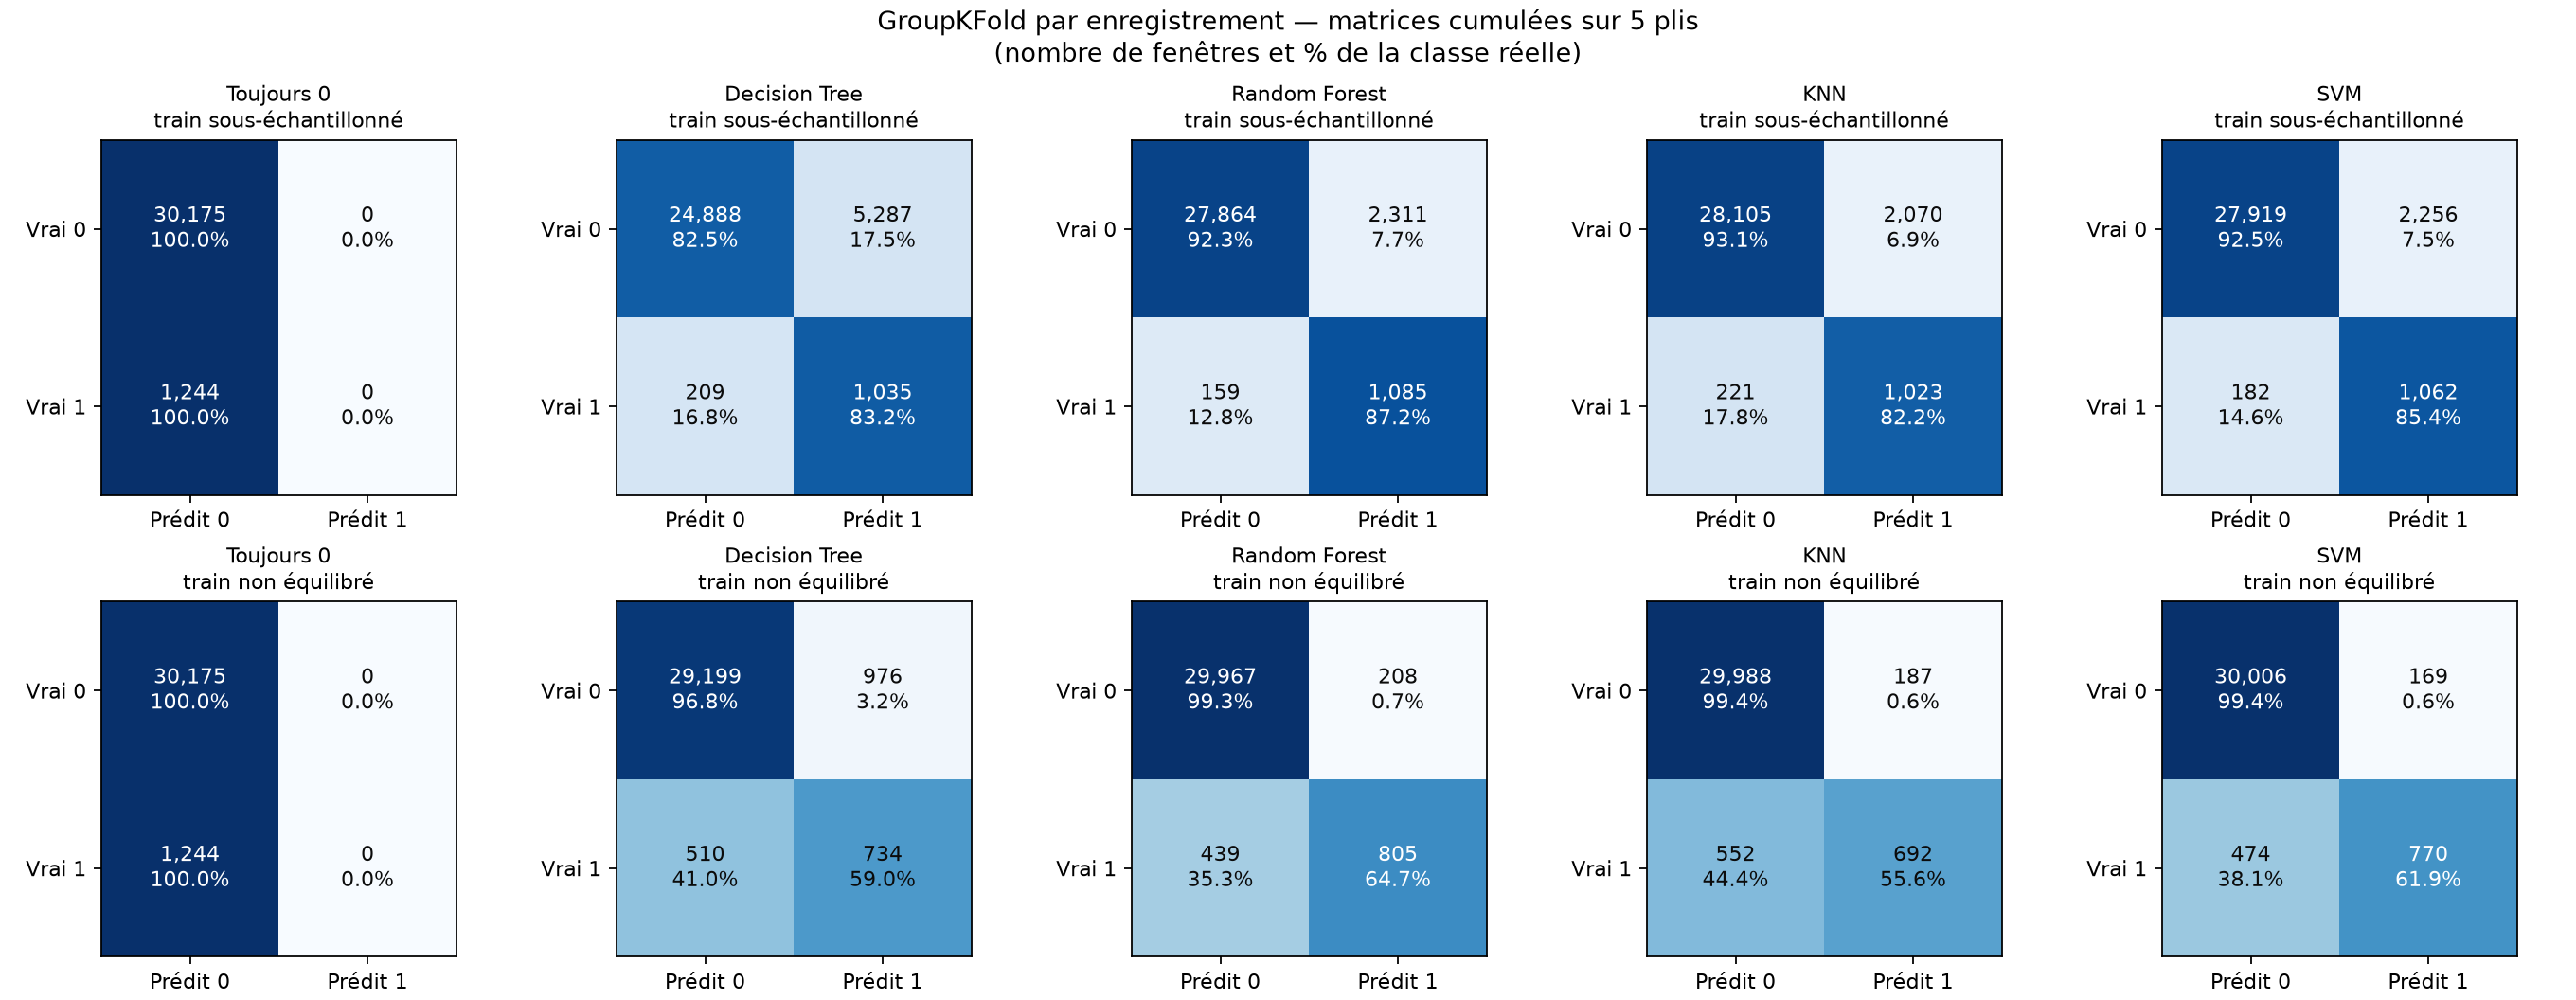
\includegraphics[width=0.95\linewidth]{official/models/confusion_matrices_groupkfold.png}
  \caption{Window-level confusion matrices for the 12 models under the \texttt{GroupKFold}
    protocol used throughout this report.}
  \label{fig:confusion-matrices}
\end{figure}

\begin{summarybox}
Twelve models --- Decision Tree, Random Forest, KNN, and SVM, each trained unbalanced, balanced,
and augmented --- were scored event by event with a recording-level 5-fold split. SVM,
unbalanced, is the best single model: event F1 0.894, 86 of 93 seizures found, 16 false alarms.
Balanced training raises recall slightly but adds far more false alarms, hurting overall F1 and
proving less stable across random seeds. A look at the best model's false alarms shows a
meaningful fraction coincide with hyperpnea or technician notes --- a real, open question about
whether some are actually unannotated seizures.
\end{summarybox}
